\section{结构化控制结构}
\hfill\ctli{实验时间}{~2014~年~11~月~30~日}
\subsection*{【实验目的】}
\begin{enumerate}[topsep=0pt,partopsep=0pt,itemsep=0pt,parsep=0pt,label={\arabic*、}]
\item 掌握基本的结构化控制结构。
\item 能够熟练进行结构化编程。
\end{enumerate}
\subsection*{【实验环境】}
\MyEnvironment
\subsection*{【实验内容】}
\begin{enumerate}[topsep=0pt,partopsep=0pt,itemsep=0pt,parsep=0pt,label={\arabic*、}]
\item 编写NumberA类,实现两个整数的加减乘除运算,可以循环计算。构造函数实现两整数a,b赋值。
\item P177:5.29
\end{enumerate}

\subsection{NumberA 类}
\subsubsection*{【详细分析】}
NumberA 类设有两个成员变量存放两个操作数,提供对这两个操作数进行四则运算的方法。

主程序循环读入两个整数,进行运算并输出。
\subsubsection*{【实验源码】}
{\linespread{1}\lstinputlisting[caption={\tt exp01.cpp}]{exp03/exp01.cpp}}
\subsubsection*{【实验结果】}
\begin{figure}[htp]
\centering
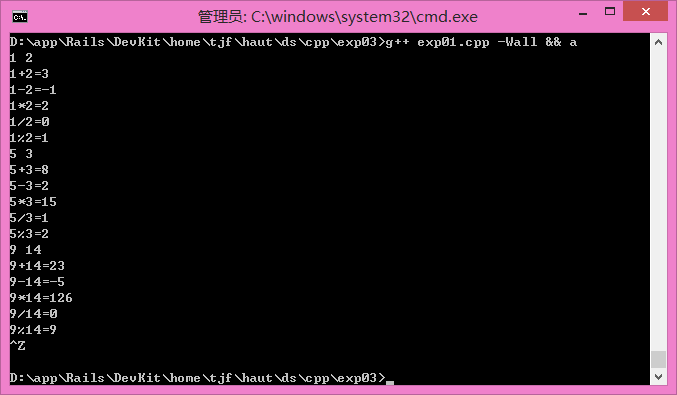
\includegraphics[width=\textwidth]{exp03/exp01.png}
\caption{\label{out03_01}NumberA 类}
\end{figure}

\subsection{P177:5.29}
\subsubsection*{【详细分析】}
用一个整数初始化类,置符号。
\subsubsection*{【实验源码】}
{\linespread{1}\lstinputlisting[caption={\tt exp02.cpp}]{exp02/exp02.cpp}}
\subsubsection*{【实验结果】}
\begin{figure}[htp]
\centering
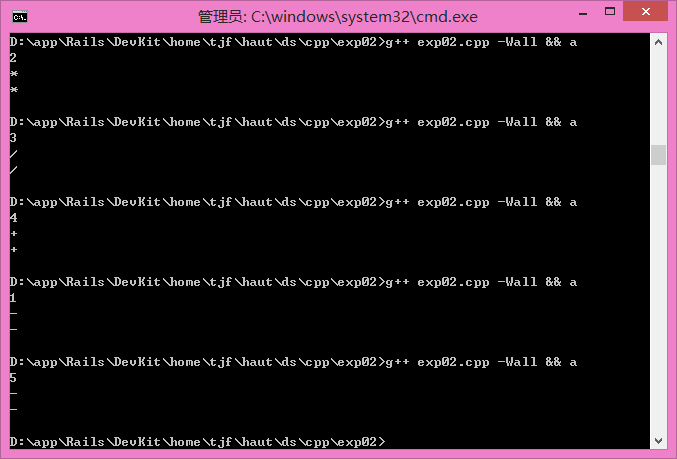
\includegraphics[width=\textwidth]{exp02/exp02.png}
\caption{\label{out03_02}P177:5.29}
\end{figure}

\subsection*{【实验体会】}
(至少150字)
